%!TEX root=paper.tex
  
  \section{Version-Aware Monitoring}
  \label{sec:version}
  
  The Stack Overflow Developer Survey from 2018 revealed the fact that 88.4\% of professional developers use Git. 
  Given that versioning using git is the main way in which the source code of services evolves and is deployed, it is natural to monitor their progress also across versions. 

  Version control in a dashboard can be supported in two ways: 
  (1) the developer explicitly states the current version, or 
  (2) the current version is automatically detected based on some version control system. 

  For \tool to start using Git, an extra configuration line enables it to automatically\footnote{Alternatively, the maintainer can add version identifiers manually for the web application through a configuration file if the system does not use Git.} associate API traffic with the currently deployed version based on information in the .git folder \footnote{\url{https://git-scm.com/}}: 
    
\begin{lstlisting}[style=custompython]

# LOC #3: provide the dashboard with 
# information on where to find the 
# git information 
dashboard.config.git = 'path/to/.git'
  
      
\end{lstlisting}  
 

  

  \subsection*{Evolving Utilization}

  \Fref{fig:mv-util} shows the \perspective{Multi-Version API Utilization} perspective which presents the utilization of the tracked endpoints across versions. The view is a matrix, in which, the intensity of the color at the intersection of an endpoint line and a version column is proportional to the percentage of requests served by that endpoint in that particular version\footnote{The chart does not plot the absolute utilization of that endpoint in that version but rather the percentage of all the API calls that go to that endpoint. Otherwise a version that is deployed for many weeks would make all those deployed for a few days invisible}.


    \begin{figure}
      \centering
      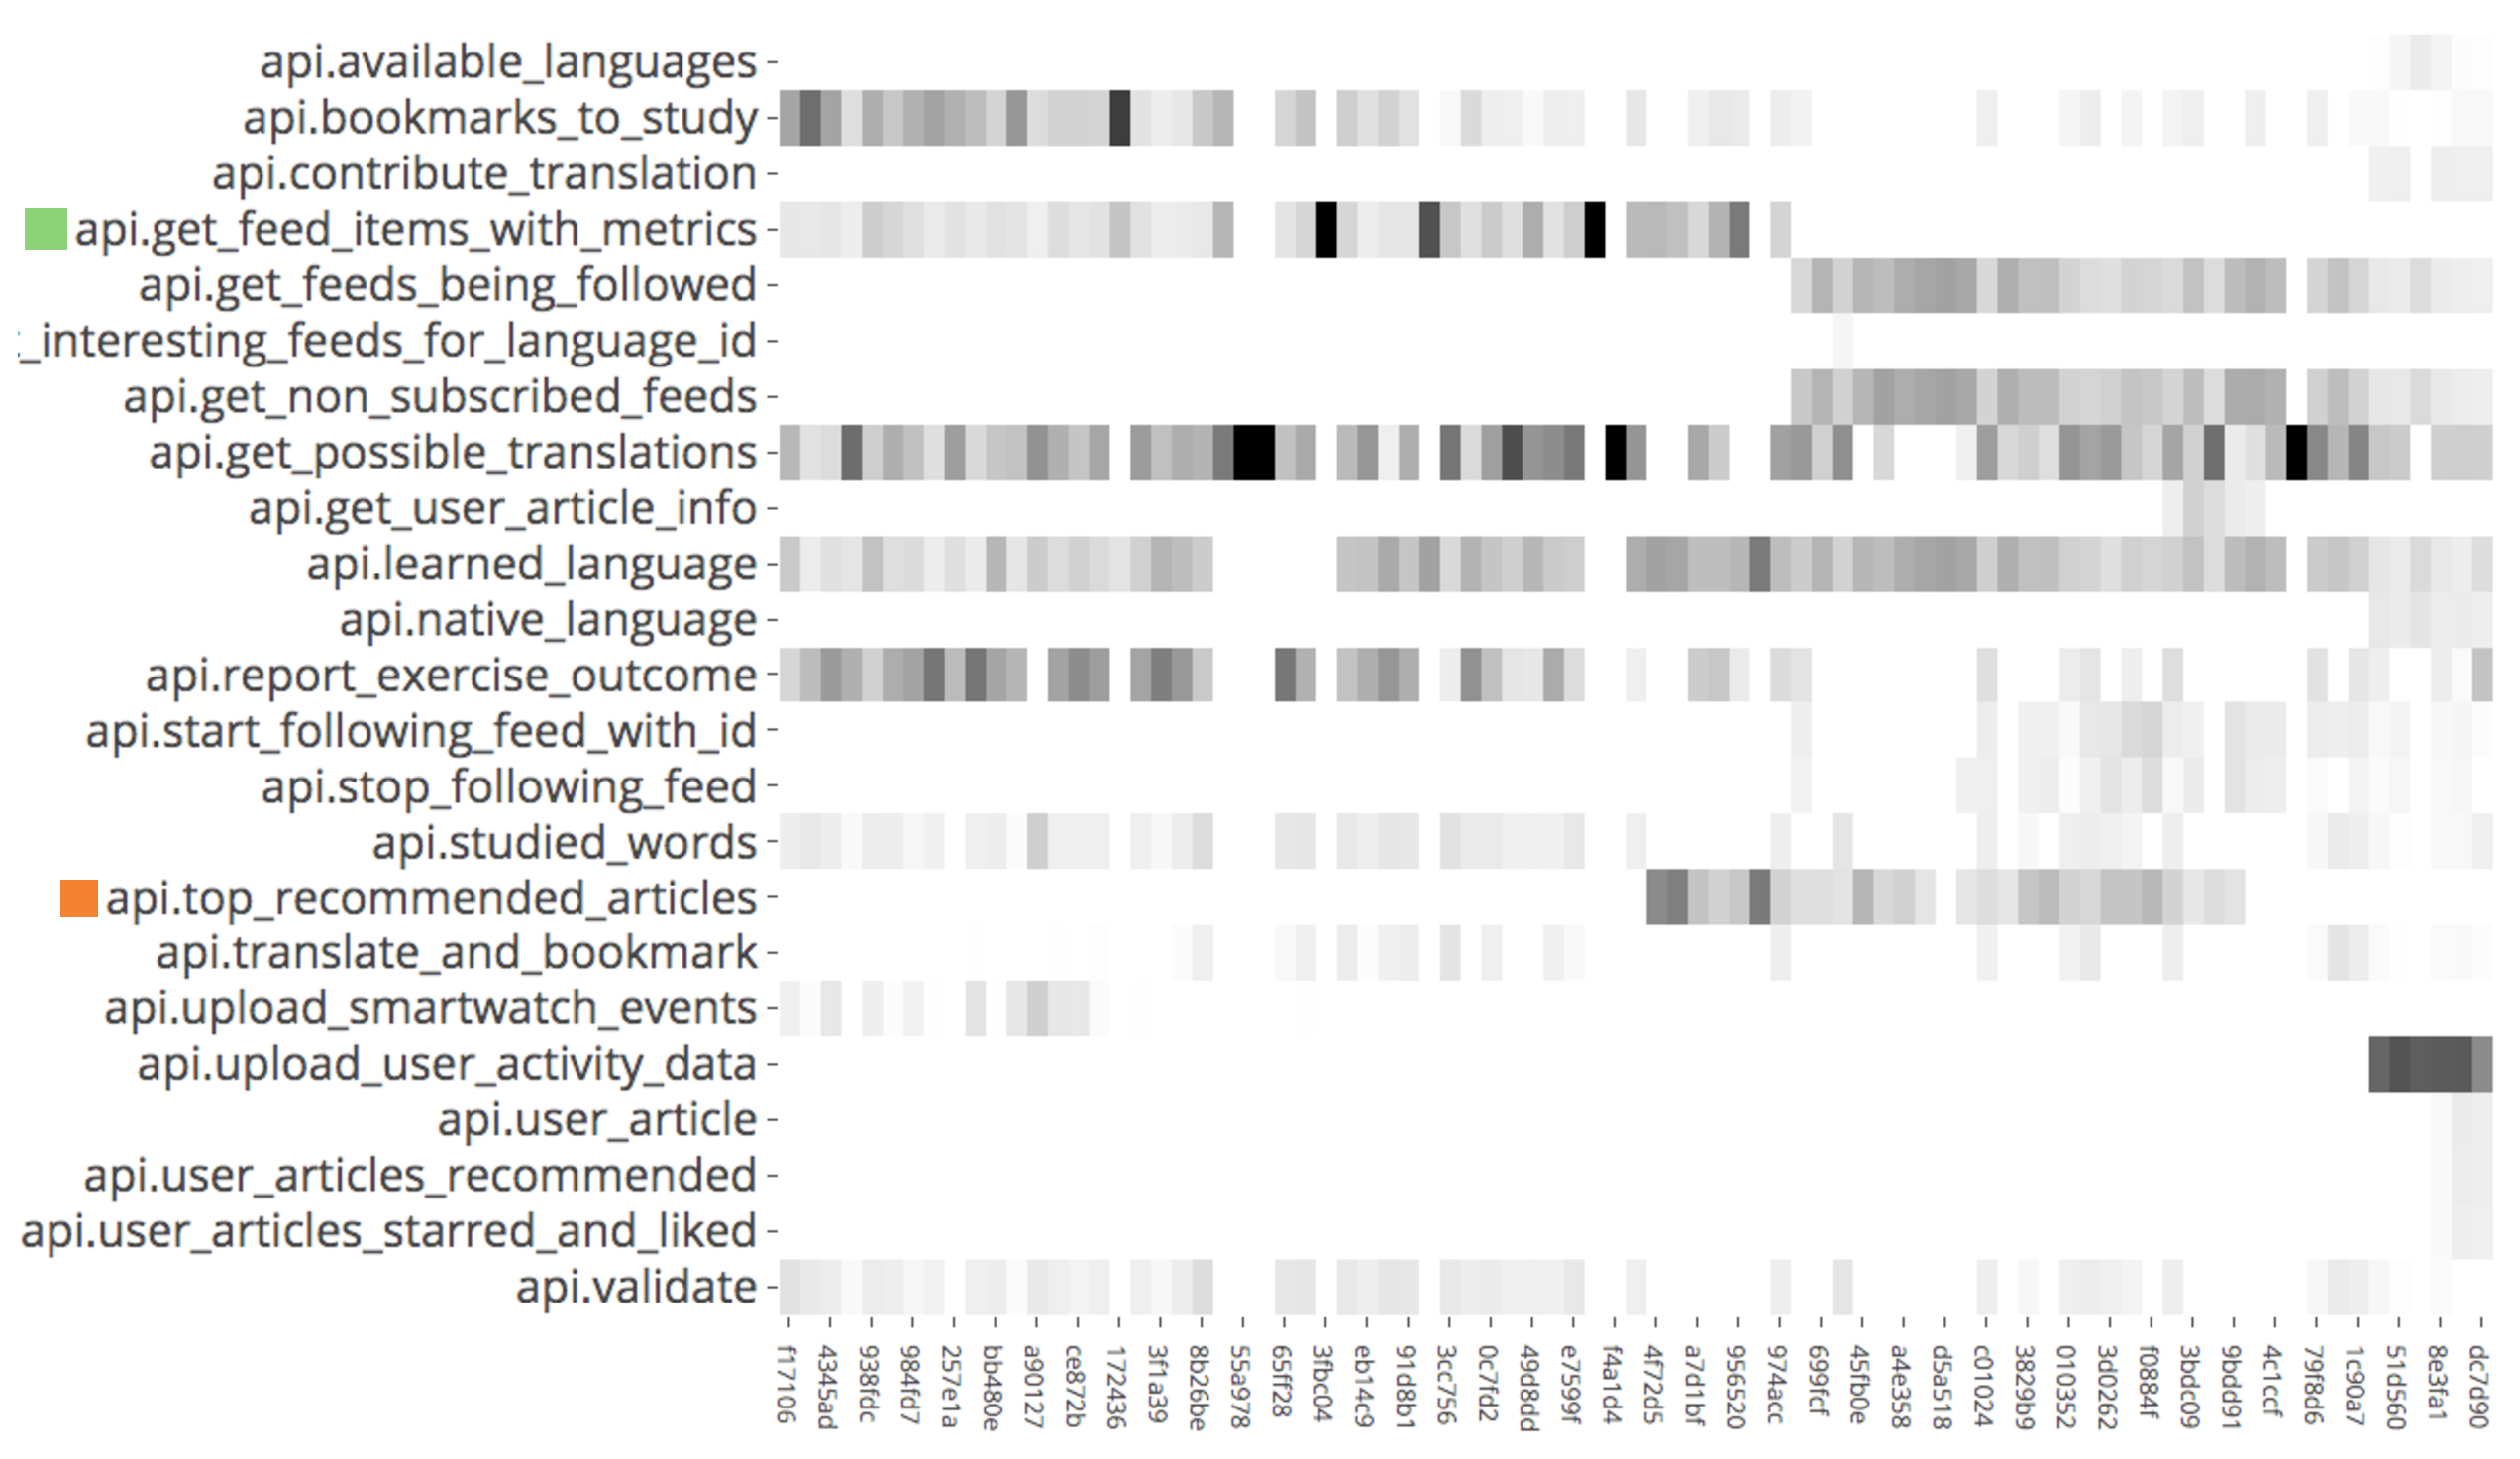
\includegraphics[width=0.9\linewidth]{utilization-evolution}
      \caption{The Evolution of All the API Endpoints Utilization Across System Versions}
      \label{fig:mv-util}
    \end{figure}

  With this view, several patterns could be visible on such a graph:
  \begin{itemize}
    
    \item Endpoints being deprecateds. In the case study \epFeedItems stops being used somewhere after the half of the presented timeline.

    \item Endpoints being introduced. In the case study, \epTopArticles appears soon after the half o the presented timeline. 

    \item Endpoint renames. Although not visible in the figure, the candidates for rename would be visible as one would discontinued at the same time when the other would appear. 

  \end{itemize}


  \subsection*{Evolving Performance}

    \Fref{fig:tee} is a zoomed-in version of such a view for \epTranslationsColor with versions increasing from top to bottom

    \begin{figure}[h!]
      \centering
      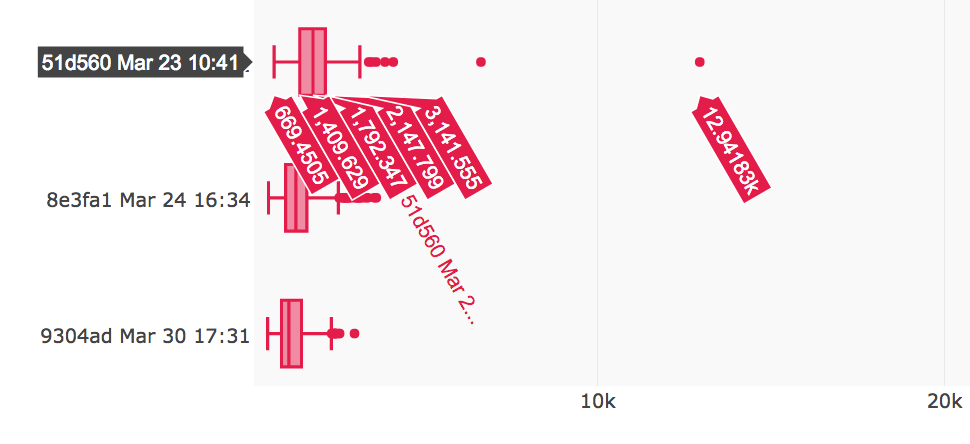
\includegraphics[width=0.9\linewidth]{translation_endpoint_evolution_}
      \caption{The Performance Evolution of the \epTranslations endpoint}
      \label{fig:tee}
    \end{figure}


  This view confirms that the performance of the translation endpoint improved in the recent versions: the median of the last three versions is constantly moving towards the left, and progresses from 1.4 seconds (in the top-most box plot in \Fref{fig:tee}) to 0.8 in the latest version (bottom-most box plot).


\subsection*{Evolving Grouped Performance}
  The limitation of the previous view is that it does not present the information also on a per user basis. To address this, a different visual perspective entitled \perspective{User-Focused Multi-Version Endpoint Performance} can be defined. \Fref{fig:tuv} presents such a perspective by mapping the average execution time for a given user (lines) and given version (columns) on the area of the corresponding circle. 

\begin{figure}[h!]
  \centering
  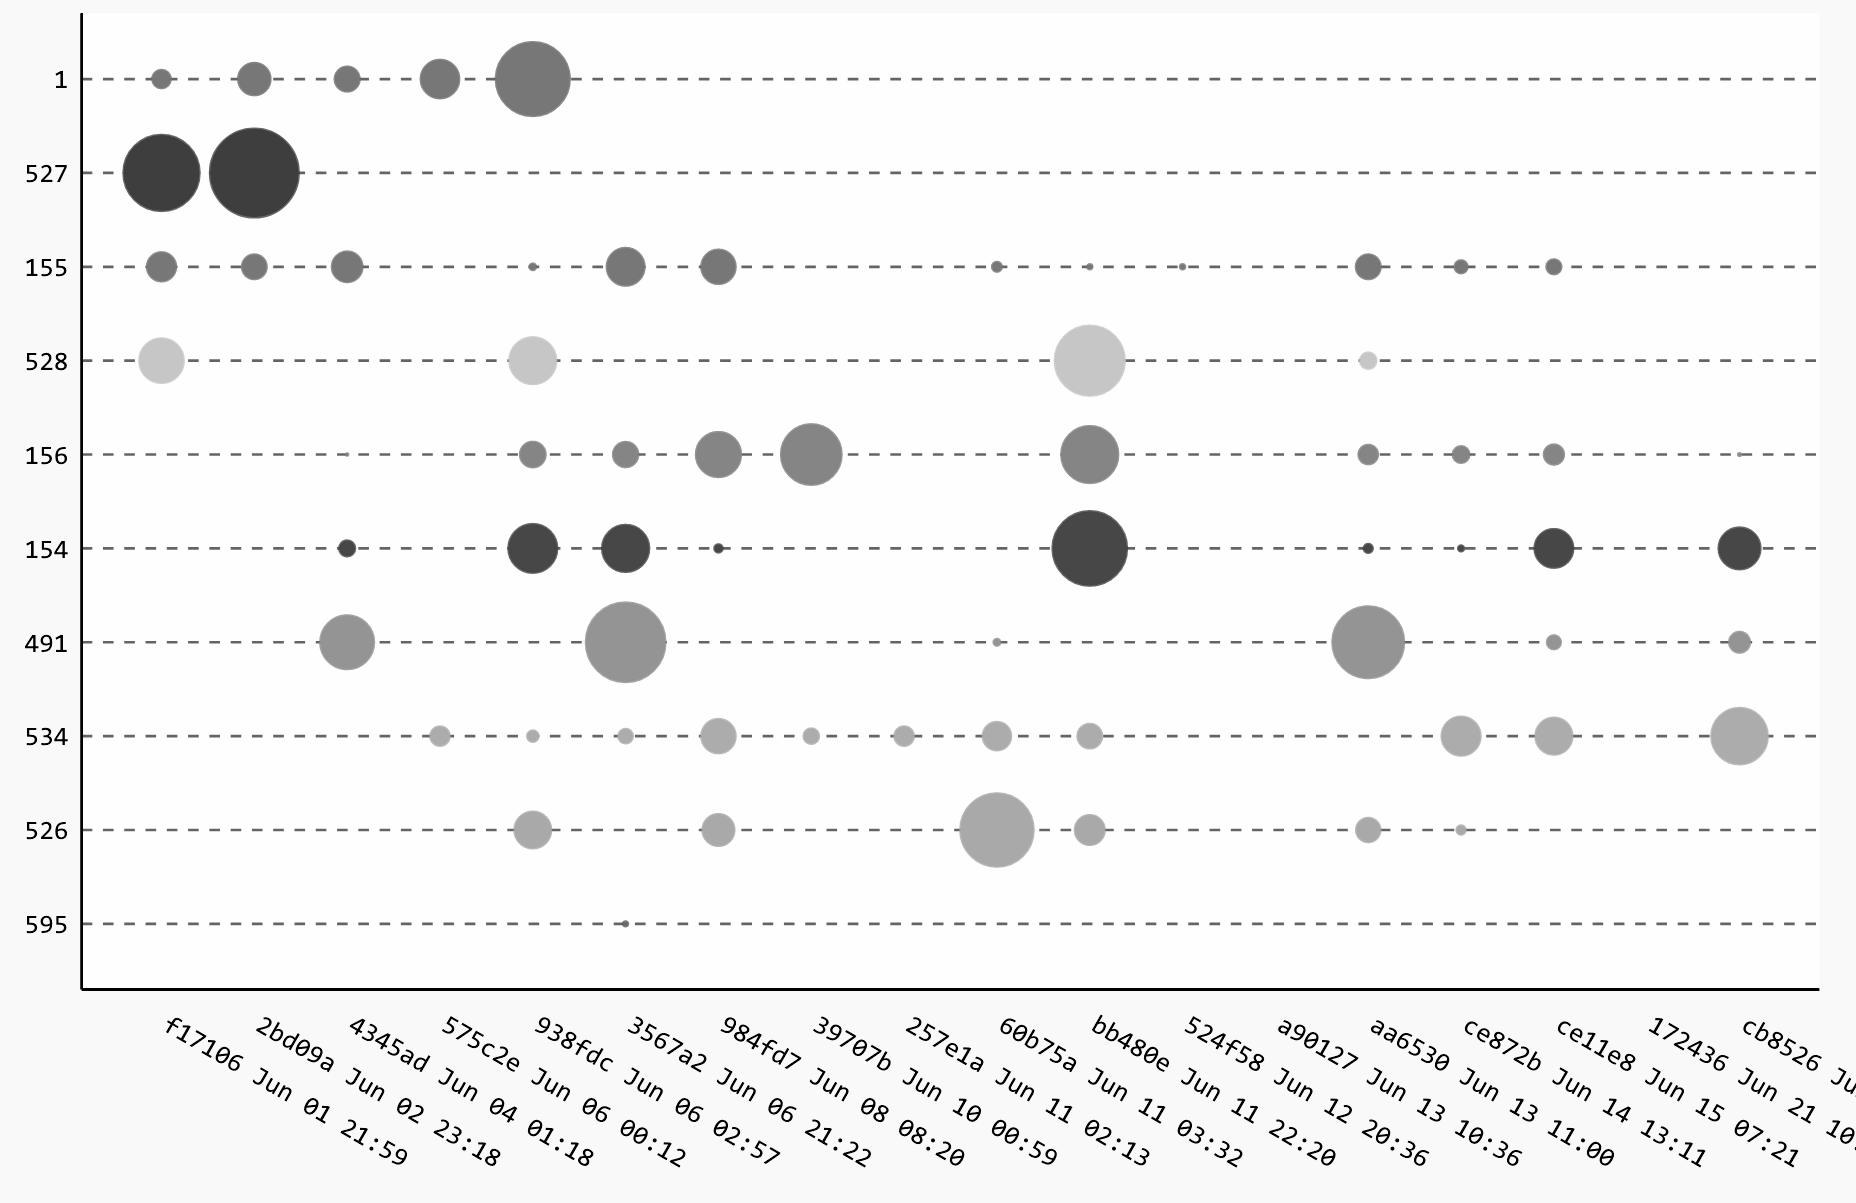
\includegraphics[width=0.77\linewidth]{time_per_user_per_version}
  \caption{This perspective shows that the evolution of response times for individual users (horizontal lines) across versions (the x-axis) for a given endpoint}
  \label{fig:tuv}
\end{figure}


The colors represent users. The figure shows average performance varying  across users and versions with no clear trend: this is probably because varying user workload (i.e. number of sources to which the user is registered) is the reason for the variation in response times. \ins{One can see that for user with id=1, performance degrades over consecutive versions. Given that for other users the performance does not degrade in the same way, it is probable that the problem might lay elsewhere: the server was overloaded or the endpoint is ``algorithmically slower''.} \va{could it be that the user kept on adding sources to their profile?}


  
